\author{Thijs Heus}
\lecture[Dynamics]{Advection, diffusion and subgrid}{dynamics}
% \section[Equations]{The LES Equations}
\begin{frame}[label=equations]{The LES Equations}
\framesubtitle<4>{Advection}
\framesubtitle<5>{Diffusion}
\framesubtitle<6>{Pressure}
\framesubtitle<7>{Other forces}
Solving velocity $\bar{u}_j$ and scalars $\bar{\phi}$ includes \memph<4>{Advection}, \memph<5>{Diffusion}, \memph<6>{Pressure} and \memph<7>{other forces and sources}.
\begin{align*}
\frac{\partial \bar{u}_i}{\partial t} & = 
&\memph<4>{- \bar{u}_j \frac{\partial \bar{u}_i}{\partial x_j} }
&\memph<6>{- c_p \Theta_0 \frac{\partial\bar{\pi}}{\partial x_i}}
&\memph<5>{+ \frac{1}{\rho_0} \frac{\partial (\rho_0 \tau_{ij})} {\partial x_j}}
&\memph<7>{ + \force{i}{} }
\\
\frac{\partial \bar{\phi}}{\partial t} & = 
&\memph<4>{ - \bar{u}_j \frac{\partial  \bar{\phi}}{\partial x_j}} 
&&\memph<5>{+ \frac{1}{\rho_0} \frac{\partial (\rho_0  \gamma_{\phi j})} {\partial x_j}}
&\memph<7>{+\source{\phi}{}}
\end{align*}
\only<2->{
Anelastic continuity $$
 \frac{\partial (\rho_0 u_i) }{\partial x_i} = 0 
$$
}
\only<3->{
Ideal gas law equation of state $$\theta_v = \theta\left[1 + (\frac{R_v}{R_d}-1)q_t - \frac{R_v}{R_d}q_l\right].$$
}
\end{frame}
\section[Time]{Timestepping}
\begin{frame}[allowframebreaks]{Timestepping}
Time stepping is based on a Runge-Kutta third order method. 

The tendencies are calculated through 3 iterations:
\begin{align*}
	\phi_*^{n} &=& \phi^{n} &+& \alpha_1 \frac{\partial \phi^{n}}{\partial t} \Delta t& \\
	\phi_{**}^{n} &=& \phi_*^{n} &+& \alpha_2 \frac{\partial \phi^{n}}{\partial t} \Delta t &+& \beta_2 \frac{\partial \phi_*^{n}}{\partial t} \Delta t \\
 	\phi^{n+1} &=& \phi_{**}^{n} &+& \alpha_3 \frac{\partial \phi_{**}^{n}}{\partial t} \Delta t &+& \beta_3 \frac{\partial \phi_*^{n}}{\partial t} \Delta t
\end{align*}
With $\alpha_i = (\frac{8}{15}, -\frac{17}{60}, \frac{3}{4})$
and $\beta_i = (0, -\frac{15}{12}, -\frac{15}{12})$.	
\pagebreak
\begin{itemize}
 \item The timestep $\Delta t$ (or \code{dt}.) in the code is variable
\item Bounded by the Courant criterion ($CFL = 0.5$)
\item Bounded by \code{dt\_long} in \code{NAMELIST}. Use it for: 
\begin{itemize}
 \item Unstabilties not in advection
 \item Unstable spin ups
 \item Circumventing bugs (but fix them later!)
\end{itemize}

\item \emph{Not} bounded by e.g. statistical timesteps. First step after $t_{samp}$ is taken for statistics; faster but slightly imprecise.
\end{itemize}
 
% % 
% The model employs a variable timestep, which is set so as to maintain
% a constant CFL maximum value bounded above by the value of the maximum
% timestep (dtlong in the NAMELIST file). If dtlong exceeds the maximum
% CFL value the actual timestep is scaled so that CFL value according
% to the new timestep is always 0.5.
\end{frame}
\section[Advection]{Advection}
\againframe<4>{equations}
\begin{frame}{Advection}

Advection can be best thought of flux through the boundaries of the cell:
\begin{align*}
 \derr{\bar{u_i}\phi_i}{x} &=& \frac{F_{i+\frac{1}{2}}-F_{i-\frac{1}{2}}}{\Delta x}
\end{align*}
 with $F_{i+\frac{1}{2}}$ the flux through the cell boundary at ${i+\frac{1}{2}}$.


\end{frame}
\begin{frame}{Advection}
\begin{center}
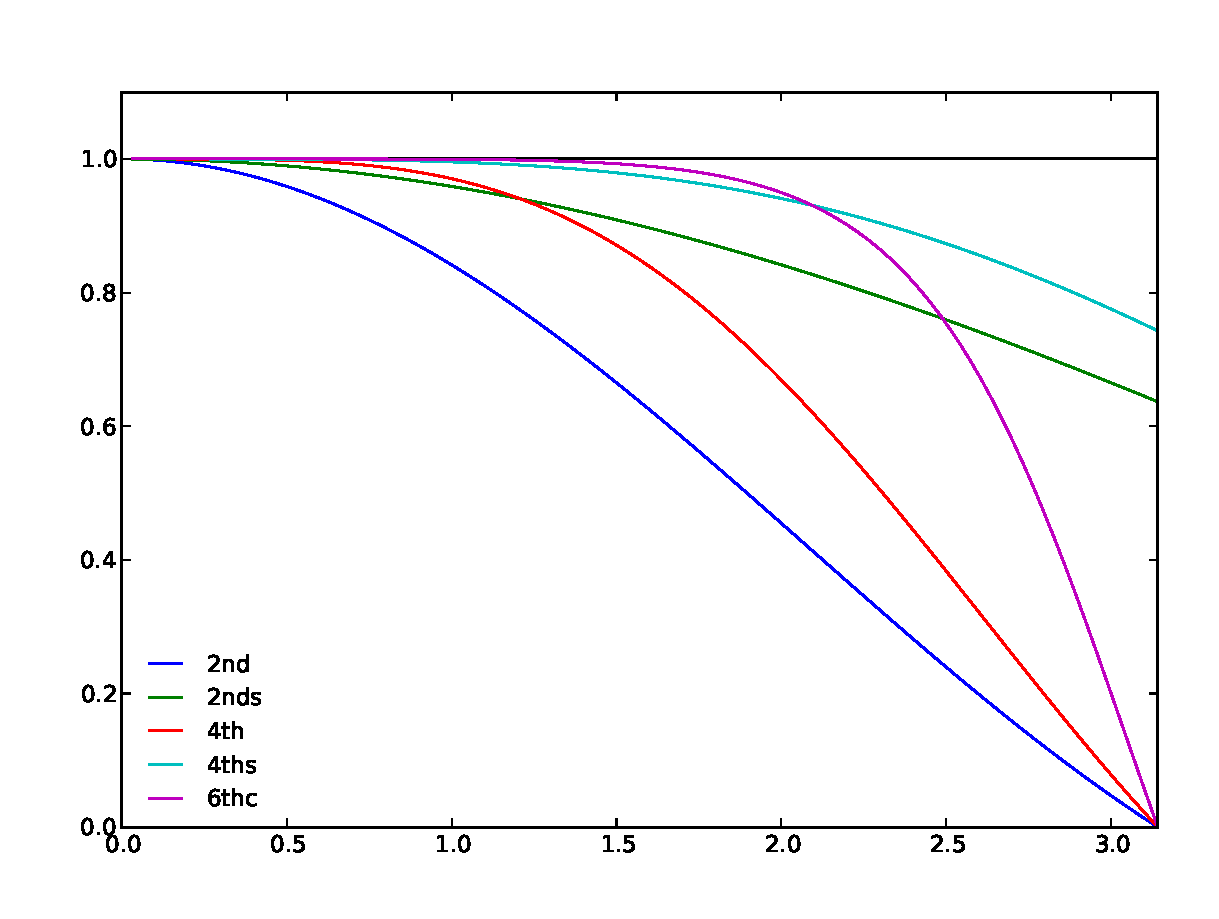
\includegraphics[height=0.7\textheight]{modkratio.pdf}       
\end{center}

\end{frame}
\begin{frame}{Advection}
\begin{center}
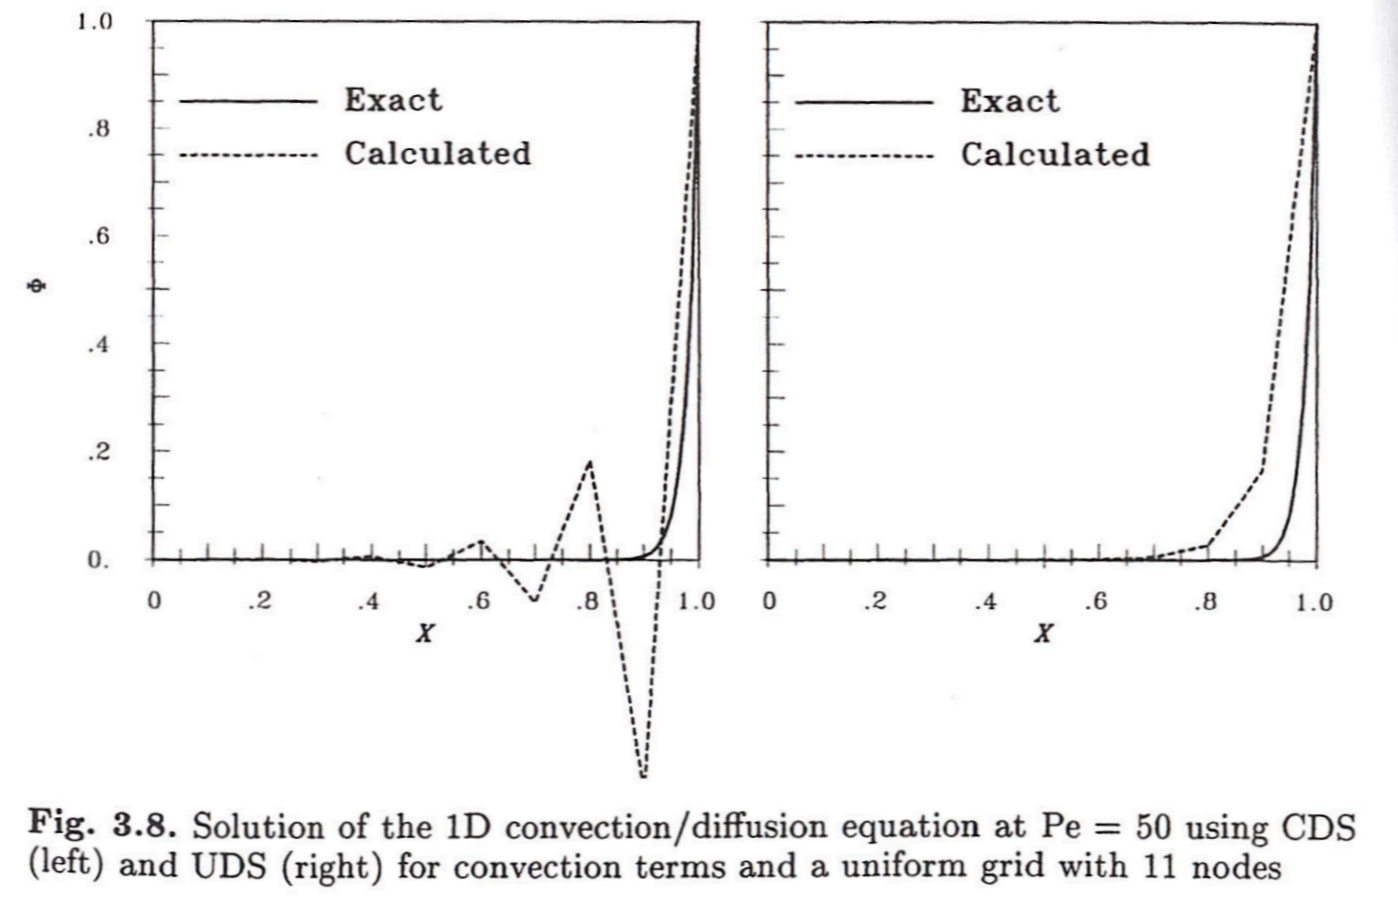
\includegraphics[height=0.7\textheight]{wiggles.png}       
\end{center}

\end{frame}

\begin{frame}{Advection}
\framesubtitle{4th order}
In UCLALES, we do 4th order Central Differencing for momentum advection, and flux-limited advection for scalars to guarantee positive values
\begin{align*}
 F^{4th}_{i+\frac{1}{2}} &=& \frac{u_{i+\frac{1}{2}}}{12} \left[-\phi_{i-1} + 7 \phi_{i} + 7 \phi_{i+1} -\phi_{i+2}\right]
\end{align*}
\pause
\begin{align*}
 F_{i+\frac{1}{2}}^{\kappa} &=& \bar{u}_{i+\frac{1}{2}} \left[\phi_{i}+\frac{1}{2}\kappa_{i+\frac{1}{2}}\left(\phi_{i}-\phi_{i-1}\right)\right]
\end{align*}
With $\kappa_{i+\frac{1}{2}} > 0 $ and a function of consecutive gradients (assuming $u_{i+\frac{1}{2}}$):
$ r = \frac{\phi_{i+1} - \phi_{i}}{\phi_{i} - \phi_{i-1}} $
\end{frame}



\begin{frame}[<+->]{Flux limiter schemes}
Depending on the setting \code{lmtr} in \code{advf.f90}, we use:
\begin{align*}
 \mathrm{\mathbf{minmod}\ } & \mathrm{min}\left(r, 1\right)  \\
 \mathrm{\mathbf{superbee}\ } & \mathrm{max}\left(\mathrm{min}\left(2 r, 1\right), \mathrm{min}\left(r, 2\right)\right)\\
 \mathrm{\mathbf{MC}\ } & \mathrm{min}(2 r,\frac{1+r}{2}, 2)  \\
 \mathrm{\mathbf{vanLeer}\ } & \frac{r + |r|}{1 + |r|}
\end{align*}
By default, it is set to MC.

Effectively, limiter schemes switch back to low order upwind schemes whenever the local gradient is to steep. 

\emph{This happens a lot in turbulent fields. This can cause so much diffusion that the SFS scheme is rendered useless}
\end{frame}

\section[Diffusion]{Diffusion}
\againframe<5>{equations}
\begin{frame}[allowframebreaks]{Diffusion}
The sub-grid fluxes $\tau_{ij}$ and $\gamma_{\phi j}$ are not known
explicitly and thus must be modeled.  This constitutes the model
closure.  The basic or default form of the closure makes use of the
Smagorinsky model, wherein
\begin{equation*}
\tau_{ij} = - \rho_0 K_mD_{ij} \quad \text{and} \quad \gamma_{\phi j}
= - \frac{K_m}{Pr} \frac{\partial \bar{\phi}} {\partial x_j},
\end{equation*}
where \[D_{ij} = \frac{\partial \bar{u}_i}{\partial x_j} +
\frac{\partial \bar{u}_j}{\partial x_i}\] is the resolved deformation,
$K_m$ is the eddy viscosity, and $Pr$ is an eddy Prandtl number.  The
Smagorinsky model calculates the eddy viscosity as
\begin{equation*}
K_m = (C_s \ell)^2 S \sqrt{1 - \frac{Ri}{Pr}} \quad \text{where} \quad
Ri =
\frac{S^2}{N^2}
\end{equation*}
and
\begin{equation*}
S^2 \equiv \frac{\partial \bar{u}_i}{\partial x_j} D_{ij} \quad
\text{and} \quad N^2 = \frac{g}{\Theta_0} \frac{\partial
\bar{\theta}_v}{\partial z}.
\end{equation*}
In the above $C_s$ is the Smagorinsky constant and takes on values
near 0.2, and
\[ \ell^{-2} = (\Delta x \Delta y \Delta z)^{-2/3} + (z\kappa/C_s)^{-2},
\]  where $\kappa=0.35$ is the von K\'arm\'an constant in the model. 
\end{frame}

\section[Pressure]{Pressure}
\againframe<6>{equations}
\begin{frame}[allowframebreaks]{Pressure(s)}
Exner function: $\bar{\pi}=(\bar{p}/p_{00})^{R_d/c_p}$ 

The anelastic approximation solves for perturbations about a
hydrostatic basic state of constant potential temperature, i.e.,
\begin{equation*}
\frac{d\pi_0}{dz} = -\frac{g}{c_p\Theta_0},
\end{equation*}
where subscript $0$ denotes a basic state value, which depend only on
$z$ ($\Theta_0$ being constant).  

For gravity, we use buoyancy deviations from the slab average (not the basic state).
For consistency, introduce a second exner $\pi_1$:

\begin{equation*}
\frac{d}{dz}(\pi_0 + \pi_1) = -\frac{g}{c_p\bar{\theta_v}},
\end{equation*}
\end{frame}
\begin{frame}{Calculating Pressure I}
Start with continuity:
\[
  \frac{\partial (\rho_0 u_i) }{\partial x_i} = 0 
\]
\pause
And the momentum equation:
\[
\frac{\partial \bar{u}_i}{\partial t}  = 
{- \bar{u}_j \frac{\partial \bar{u}_i}{\partial x_j} }
{- c_p \Theta_0 \frac{\partial\bar{\pi}}{\partial x_i}}
{+ \frac{1}{\rho_0} \frac{\partial (\rho_0 \tau_{ij})} {\partial x_j}}
{ + \force{i}{} } 
\]
\pause
Fill them in in each other:
\[
\derr{}{x_i}\left(\rho_0\frac{\partial \bar{u}_i}{\partial t}\right)   =\derr{}{x_i}\left[
- \rho_0\bar{u}_j \frac{\partial \bar{u}_i}{\partial x_j} 
- \rho_0 c_p \Theta_0 \frac{\partial\bar{\pi}}{\partial x_i}
+ \frac{\partial (\rho_0 \tau_{ij})} {\partial x_j}
{ + \rho_0\force{i}{} }\right] = 0
\]
\end{frame}
\begin{frame}{Calculating Pressure II}
\[
\derr{}{x_i}\left[
- \rho_0\bar{u}_j \frac{\partial \bar{u}_i}{\partial x_j} 
- \rho_0 c_p \Theta_0 \frac{\partial\bar{\pi}}{\partial x_i}
+ \frac{\partial (\rho_0 \tau_{ij})} {\partial x_j}
{ + \rho_0\force{i}{} }\right] = 0
\]
Bring the pressure to the other side:
\[
\derr{}{x_i}\left(\rho_0{ c_p \Theta_0 \frac{\partial\bar{\pi}}{\partial x_i}}\right)   = \derr{}{x_i}\left[
- \rho_0\bar{u}_j \frac{\partial \bar{u}_i}{\partial x_j} 
+ \frac{\partial (\rho_0 \tau_{ij})} {\partial x_j}
{ + \rho_0\force{i}{} }\right] 
\]
\pause
And we end up with a Poisson equation:
\[
\derr{}{x_i}\left(\rho_0{\frac{\partial\bar{\pi}}{\partial x_i}}\right)   = \frac{1}{ c_p \Theta_0 }\derr{}{x_i}\left[
- \rho_0\bar{u}_j \frac{\partial \bar{u}_i}{\partial x_j} 
+ \frac{\partial (\rho_0 \tau_{ij})} {\partial x_j}
{ + \rho_0\force{i}{} }\right] 
\]
that can be solved efficiently (but globally!) in Fourier space.
\end{frame}
